\documentclass{beamer}
\usepackage[orientation=portrait,size=a2,scale=1.3]{beamerposter}
\mode<presentation>{\usetheme{ZH}}
\usepackage[utf8]{inputenc}
\usepackage{booktabs}
\usepackage{array,tabularx}
\usepackage{hyperref}
\usepackage{ragged2e}
% One smaller size for tables, captions and references; nothing else.
\usepackage[font=small,justification=justified]{caption}
\usepackage{helvet}
\newcolumntype{Z}{>{\centering\arraybackslash}X}

\title{\huge Zero-Day Detection under\\ HAI Plant-Version Shift}
\author{Hongbin Zhang, Zeren Wang}
\institute[Chalmers]{Project Group 88 \,\textbullet\, SSY340 Deep Machine Learning \,\textbullet\, Chalmers University of Technology}
\date{\today}

\newlength{\columnheight}
\setlength{\columnheight}{46cm}

\begin{document}
\begin{frame}
\begin{columns}

% ============================== COLUMN 1 ==============================
\begin{column}{.30\textwidth}
\begin{beamercolorbox}[center]{postercolumn}
\begin{minipage}{.98\textwidth}
\parbox[t][\columnheight]{\textwidth}{

\begin{myblock}{The problem}
A zero-day detector must flag attacks it has never seen, trained on normal
operation alone. The harder case is when the \emph{plant itself} is replaced by a
later, differently instrumented version: HAI 21.03 and 23.05 are two such versions
of the same testbed, sharing 59 tags but not the instrumentation.

\vspace{0.3cm}
\textbf{How much does detection degrade from 21.03 to 23.05, and can an adaptive
decision layer recover what is lost?}

\vspace{0.3cm}
Thresholds are the obvious suspect. A detector that alarms at a fixed rate on one
plant version will alarm at a different rate on the next, and an operator cannot
re-tune it by hand. If the representation still separates attacks from normal
operation, a threshold that follows the stream should recover the loss. If it does
not, no threshold can.
\end{myblock}\vfill

\begin{myblock}{Data and protocol}
\begin{center}
\small
\begin{tabular}{@{}lrrr@{}}
\toprule
\textbf{partition} & \textbf{files} & \textbf{rows} & \textbf{attacks} \\
\midrule
21.03 normal training & 3 & 921,603 & 0 \\
21.03 test & 5 & 402,005 & 50 \\
23.05 test & 2 & 284,400 & 52 \\
\bottomrule
\end{tabular}
\end{center}

\vspace{0.3cm}
The two versions share 59 public tags; 18 have zero variance throughout the normal
21.03 training data and are removed \emph{using source statistics only}, leaving
\textbf{41 modelling tags}. Their constant source encoding would otherwise dominate
max-fused scores after the shift.
\end{myblock}\vfill

\begin{myblock}{Protocol}
\begin{itemize}
  \item \textbf{No attack labels} are used for training, model selection, or
        threshold calibration.
  \item Normalisation is fitted on chronological 21.03 training partitions; the last
        15\% supplies normal calibration scores.
  \item EVT is calibrated on \textbf{source-normal} scores to an empirical target of
        \textbf{10 false alarms/day}. Three seeds (11, 23, 37); no point adjustment.
\end{itemize}
\end{myblock}

}\end{minipage}\end{beamercolorbox}
\end{column}

% ============================== COLUMN 2 ==============================
\begin{column}{.325\textwidth}
\begin{beamercolorbox}[center]{postercolumn}
\begin{minipage}{.98\textwidth}
\parbox[t][\columnheight]{\textwidth}{

\begin{myblock}{Three detectors}
\begin{itemize}
  \item \textbf{PCA} --- reconstruction error on flattened windows.
  \item \textbf{Deep SVDD} --- a bias-free 1-D CNN trunk into a latent hypersphere
        (13{,}904 parameters).
  \item \textbf{Convolutional VAE} --- the same trunk plus Gaussian heads and a
        decoder (26{,}352 parameters).
\end{itemize}

\vspace{0.2cm}
Causal 60\,s windows, scored at the window end, 10\,s evaluation stride. Per-sensor
scores are fused by \textbf{maximum}, so an alarm needs one strongly anomalous
sensor. The two neural models share the trunk but not the total parameter count, and
that gap is reported rather than hidden.
\end{myblock}\vfill

\begin{myblock}{Result 1: in-domain, at 10 alarms/day}
\begin{center}
\small
\begin{tabular}{@{}lrrrr@{}}
\toprule
& \textbf{event recall} & \textbf{eTaF1} & \textbf{PR-AUC} & \textbf{Hit@3} \\
\midrule
PCA & 0.740 & 0.533 & 0.502 & 0.229 \\
Deep SVDD & \textbf{0.773} & \textbf{0.543} & 0.489 & 0.171 \\
VAE & 0.560 & 0.473 & 0.462 & \textbf{0.257} \\
\bottomrule
\end{tabular}
\end{center}

\vspace{0.2cm}
At 10 false alarms per day on 21.03 all three work moderately --- and none of them
works well. A PR-AUC near 0.5 at a 1--2\% attack rate is a weak ranker: there was
little left to lose.
\end{myblock}\vfill

\begin{myblock}{Result 2: the representation collapses}
\begin{figure}
\centering
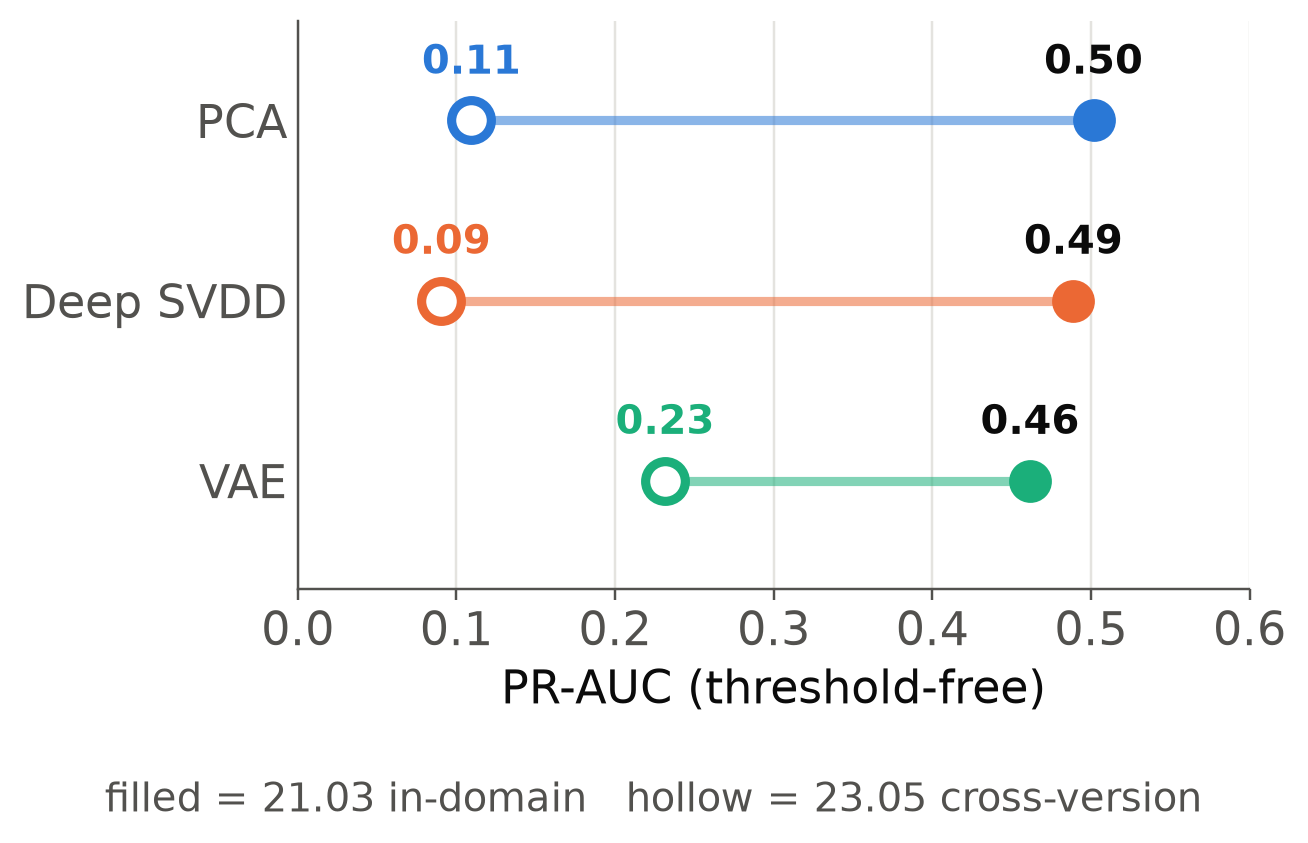
\includegraphics[width=0.96\linewidth]{fig/fig_prauc.png}
\caption{PR-AUC is threshold-free, so it measures the representation alone.}
\end{figure}

\vspace{0.1cm}
PCA 0.50 $\to$ 0.11, Deep SVDD 0.49 $\to$ 0.09, VAE 0.46 $\to$ 0.23. VAE retains the
most; PCA and Deep SVDD retain almost nothing.
\end{myblock}

}\end{minipage}\end{beamercolorbox}
\end{column}

% ============================== COLUMN 3 ==============================
\begin{column}{.325\textwidth}
\begin{beamercolorbox}[center]{postercolumn}
\begin{minipage}{.98\textwidth}
\parbox[t][\columnheight]{\textwidth}{

\begin{myblock}{Result 3: recall 1.000 is alarm collapse}
\begin{figure}
\centering
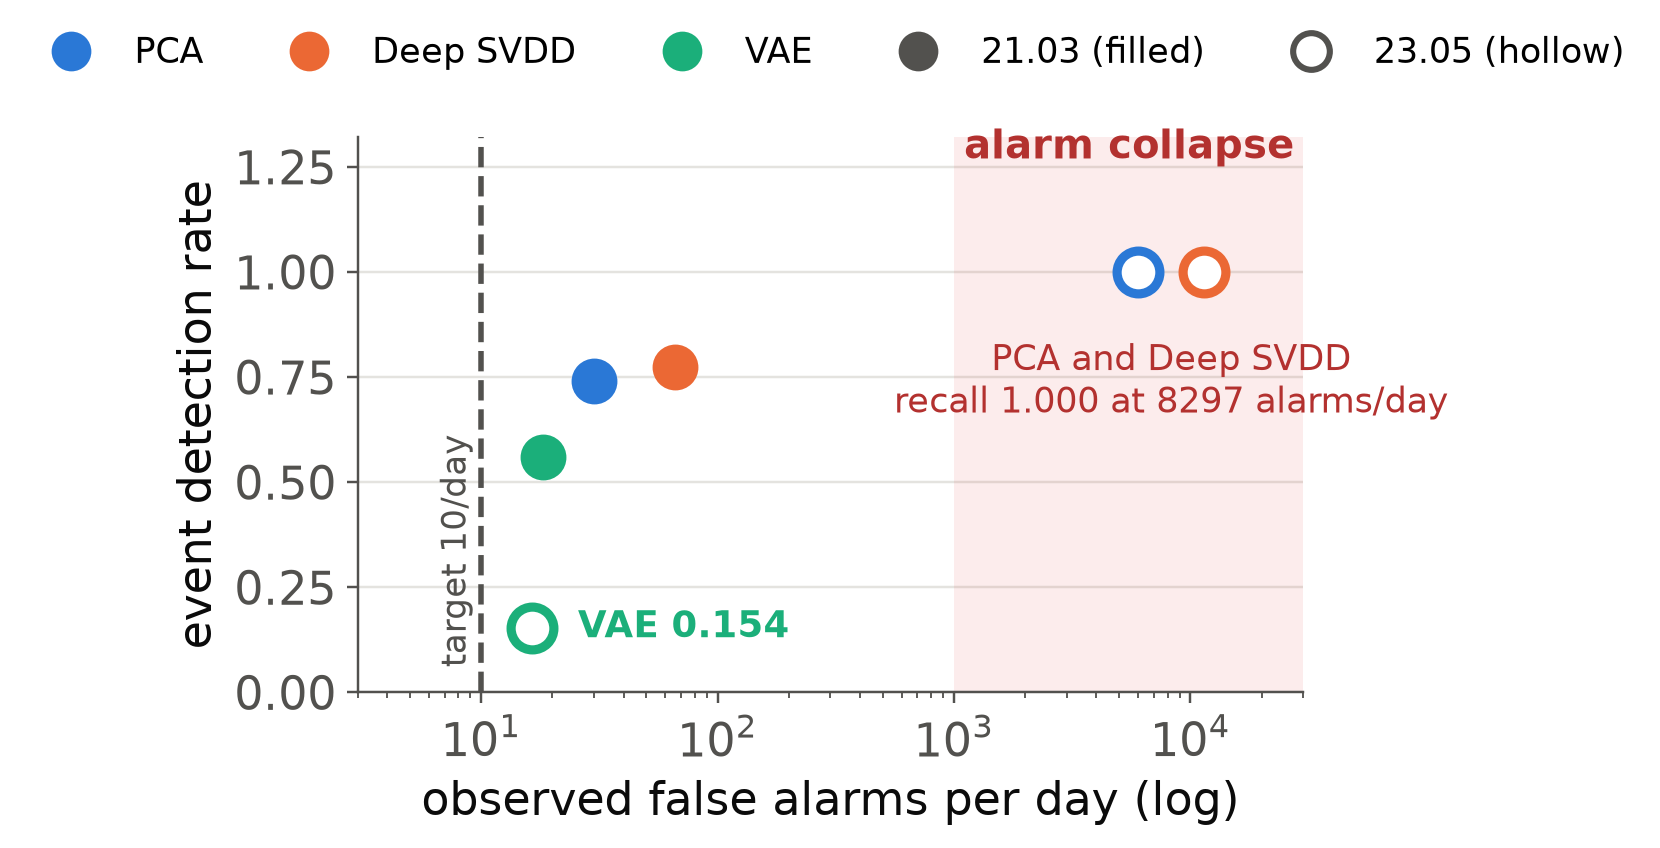
\includegraphics[width=0.96\linewidth]{fig/fig_collapse.png}
\caption{Frozen arm; the calibration target was 10 alarms/day.}
\end{figure}

\vspace{0.1cm}
On 23.05, PCA and Deep SVDD report \textbf{event recall 1.000} because they fire
\textbf{8,297 alarms per day}, on 96\% of normal windows. A circular-shift null
settles it: a randomly time-shifted alarm series matches this recall in 200 of 200
shifts ($p=1.00$), while on 21.03 the same models beat their null at $p<0.001$.
\end{myblock}\vfill

\begin{myblock}{Result 4: DSPOT cannot recover it}
\begin{center}
\small
\begin{tabular}{@{}lrrrr@{}}
\toprule
\textbf{model} & \textbf{frozen} & \textbf{adaptive} & \textbf{gain} & \textbf{FA/day} \\
 & \multicolumn{2}{c}{\emph{23.05 event recall}} & & \emph{frozen$\to$adapt.} \\
\midrule
PCA & 1.000$^\dagger$ & 1.000$^\dagger$ & 0.000 & 8297$\to$8297 \\
Deep SVDD & 1.000$^\dagger$ & 1.000$^\dagger$ & 0.000 & 8297$\to$8297 \\
VAE & 0.154 & 0.115 & \textbf{$-$0.038} & 16.4$\to$5.5 \\
\bottomrule
\end{tabular}

\vspace{0.15cm}
{\small $^\dagger$Alarm collapse: a circular-shift null reaches 1.000 in 200/200
shifts ($p=1.00$). Not detection.}
\end{center}

\vspace{0.1cm}
\textbf{Why.} PR-AUC is \emph{identical} across arms: both threshold the same scores.
DSPOT moves the threshold, not the encoder, the PCA basis, or the score.
\end{myblock}\vfill

\begin{myblock}{Conclusions}
\begin{itemize}
  \item \textbf{Decision-layer adaptation cannot substitute for representation
        quality.} DSPOT helps where the representation still works and does nothing
        where it does not.
  \item \textbf{Zero-day detection does not survive the version shift.} Ranking
        quality falls four- to five-fold; two of three detectors collapse into
        continuous alarm.
  \item \textbf{Report threshold-free metrics beside event recall}: recall 1.000 and
        0.154 can describe equally useless detectors.
  \item Limits: one testbed, two versions, three seeds; the source calibration
        targets an empirical source rate, not a guaranteed shifted-domain budget.
\end{itemize}
\end{myblock}\vfill

\begin{myblock}{References}
{\small
[1] H.-K. Shin et al. \emph{HAI: HIL-based Augmented ICS Security Dataset}. CSET 2020.\\{}
[2] L. Ruff et al. \emph{Deep One-Class Classification}. ICML 2018.\\{}
[3] L. Ruff et al. \emph{Rethinking Assumptions in Deep Anomaly Detection}. arXiv:2006.00339, 2020.\\{}
[4] A. Siffer et al. \emph{Anomaly Detection in Streams with Extreme Value Theory}. KDD 2017.\\{}
[5] W.-S. Hwang et al. \emph{Time-Series Aware Precision and Recall for Anomaly Detection}. CIKM 2019.\\{}
[6] W.-S. Hwang et al. \emph{Do You Know Existing Accuracy Metrics Overrate Time-Series Anomaly Detections?} SAC 2022.\\{}
[7] S. Kim et al. \emph{Towards a Rigorous Evaluation of Time-series Anomaly Detection}. AAAI 2022.
}
\end{myblock}

}\end{minipage}\end{beamercolorbox}
\end{column}

\end{columns}
\end{frame}
\end{document}
